\section{Helical plateaux, toroidal bodies, and exterior compatibility}
\label{sec:topology-exterior}

The outer problem has two independent global features. Positivity can force a
constant-$\eta$ region before infinity is reached, while an axis-avoiding
compact body naturally has toroidal rather than simply connected exterior
topology. Neither feature is visible in a purely local matching calculation.

\subsection{Eventual vacuum and the helical flat quotient}

\begin{theorem}[Eventual vacuum and helical plateau]
\label{thm:eventual-helical-plateau}
Let a constant-$\ellzero\neq0$ regular sheet reach an asymptotically flat
end and obey the uniform subluminality hypothesis of
Corollary~\ref{cor:exact-asymptotic-decay}. Suppose $\rho\geqslant0$ on an
open neighbourhood of every sufficiently large point of the sheet. Then
$\eta$ is constant on an outer open set and $\rho=0$ there. If that set lies
in the same connected invertible sheet as the interior, then $\eta$ is
constant on the entire sheet. After asymptotic normalization, the plateau
metric is
\begin{equation}
ds^2=-(dt-q_0\,d\phi)^2+r^2d\phi^2+dr^2+dz^2,
\qquad \phi\sim\phi+2\pi,
\label{eq:helical-plateau-metric}
\end{equation}
where $q_0$ is the locking constant in
Eq.~\eqref{eq:asymptotic-locking-q}.
\end{theorem}

\begin{proof}
The asymptotic decay $v=O(r^{-1})$ makes both endpoints of the density
interval in Eq.~\eqref{eq:density-domain} tend to zero, whereas
$r\ellzero$ is unbounded. The algebraic density factor is therefore
negative at every sufficiently large point. Since the full density is
assumed nonnegative in a neighbourhood, Corollary~\ref{cor:vacuum-plateau}
forces $\nabla\eta=0$ and $\rho=0$ on a neighbourhood of each such point.
Theorem~\ref{thm:automatic-analyticity} propagates the resulting plateau
through the connected invertible sheet.

On a constant-$\eta$ region, $H$ and $\Omega$ are constant and the
reconstruction quadratures make $\mu$ constant. Asymptotic normalization
sets $H=-1$, $\Omega=0$, and $\mu=0$. Substitution into
Eq.~\eqref{eq:model-metric-components} gives
$g_{tt}=-1$, $g_{t\phi}=q_0$, and
$g_{\phi\phi}=r^2-q_0^2$, which is precisely
Eq.~\eqref{eq:helical-plateau-metric}.
\end{proof}

\begin{corollary}[Regular-axis exclusion of a nontrivial helical plateau]
\label{cor:helical-regular-axis-exclusion}
Under the hypotheses of Theorem~\ref{thm:eventual-helical-plateau}, suppose
the plateau metric extends within the same connected flat
stationary-axisymmetric region to a regular fixed point of the axial action.
Then $q_0=0$. If the positive dust sheet itself reaches the end, this
contradicts the required locking value $q_0=q>0$. Thus a nonzero helical
plateau can occur only on an axis-excised region or behind a change of
domain, equations, or regularity; it is not a standard connected
regular-axis completion of the dust sheet.
\end{corollary}

\begin{proof}
At a regular fixed point, $g(m,m)=0$ and the orbit-area radius is $r=0$.
The continued identity
$g(m,m)=r^2-q_0^2$ therefore gives $q_0=0$. For a positive dust sheet that
itself reaches the end, Theorem~\ref{thm:exact-asymptotic-locking} gives
$q_0=q>0$. The two conclusions are incompatible.
\end{proof}

On the universal cover, $T=t-q_0\phi$ makes
Eq.~\eqref{eq:helical-plateau-metric} Minkowskian. The deck transformation
acts by
$$
(T,\phi)\longmapsto(T-2\pi q_0,\phi+2\pi).
$$
Thus the Lorentz holonomy is trivial but the affine time-translation
holonomy is nonzero when $q_0\neq0$. The cylinder $r=|q_0|$ is a chronology
cylinder, not a horizon. An actual outer plateau restricted to
$r>r_0>|q_0|$ is stably causal because $g^{tt}<0$ there; closed azimuthal
timelike curves arise only in an inward extension to $r<|q_0|$. This is a
helical flat quotient, geometrically the zero-deficit member of the usual
spinning-string family, but no string source has been constructed.

\subsection{Toroidal topology and period obstructions}

\begin{theorem}[Topology of an axis-avoiding compact body]
\label{thm:toroidal-body-periods}
Let a spacelike slice carry an effective regular axial $U(1)$ action with no
exceptional orbits in the region considered, and let its orbit surface be a
half-plane. Suppose a compact connected invariant matter body projects to a
smoothly embedded closed disk $B\Subset\{r>0\}$. Then
$$
\Omega_{\rm mat}\simeq D^2\times S^1,
\qquad
\partial\Omega_{\rm mat}\simeq T^2,
$$
and the vacuum orbit surface
$Q^+=Q\setminus\operatorname{int}B$ satisfies
$$
\pi_1(Q^+)\simeq\mathbb Z,
\qquad
H^1_{\rm dR}(Q^+)\simeq\mathbb R.
$$
Let $q$ denote the vacuum orbit metric and
$\varpi=\sqrt{-\det G}$. A global Weyl conjugate $\zeta$ and a global twist
potential $\chi$ exist exactly when
\begin{equation}
P_\zeta:=\oint_\gamma *_q d\varpi=0,
\qquad
P_\chi:=\oint_\gamma\omega_k=0
\label{eq:topological-period-tests}
\end{equation}
for a generator $\gamma$ of $H_1(Q^+;\mathbb Z)$. Even when both periods
vanish, global Weyl coordinates additionally require $d\varpi\neq0$ and
global injectivity and properness of $(\varpi,\zeta)$.
\end{theorem}

\begin{proof}
The circle action is free over $B$. Its principal circle bundle is trivial
because $H^2(D^2;\mathbb Z)=0$, proving the solid-torus and boundary
statements. The half-plane with the interior of one embedded disk removed
deformation retracts onto a circle, which proves the homotopy and de Rham
claims. In vacuum, $*_q d\varpi$ and the descended twist form $\omega_k$ are
closed. A closed one-form on $Q^+$ is exact precisely when its period on the
single homology generator vanishes. Exactness supplies single-valued
potentials, while noncriticality and global one-to-one proper behaviour are
the separate conditions needed for those potentials to be coordinates.
\end{proof}

\begin{figure*}[t]
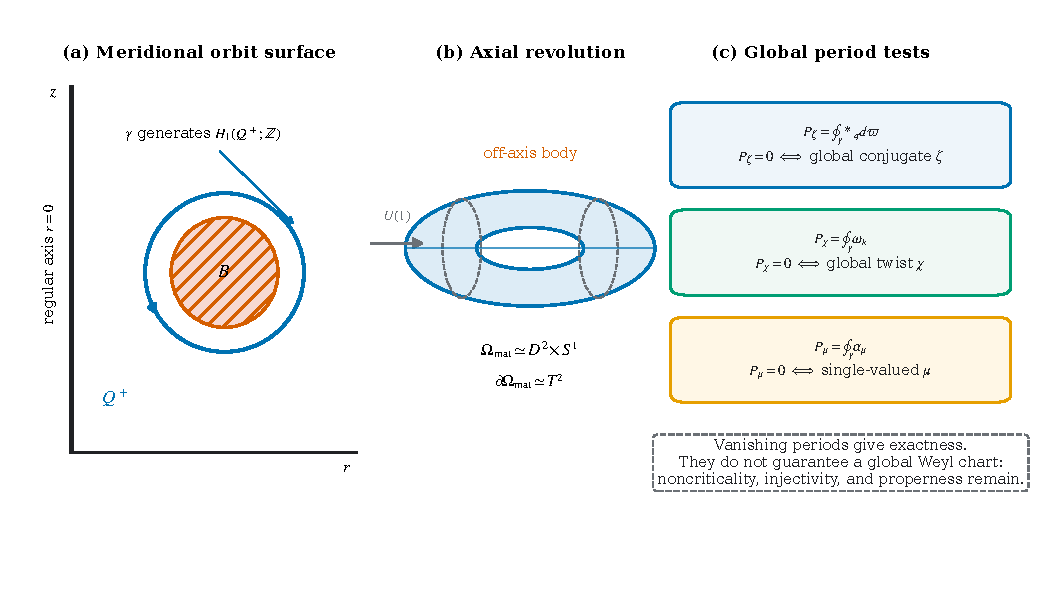
\includegraphics[width=\textwidth]{figures/toroidal_period_obstructions.pdf}
\caption{Topology and periods for one compact axis-avoiding body. Its
meridional disk $B$ revolves to
$\Omega_{\rm mat}\simeq D^2\times S^1$, while the exterior orbit surface
$Q^+$ has one homology generator $\gamma$. Under the local closedness
equations, $P_\zeta=0$, $P_\chi=0$, and $P_\mu=0$ are exactly the
single-valuedness tests for $\zeta$, $\chi$, and $\mu$, respectively. The
first two period tests still do not make $(\varpi,\zeta)$ a global Weyl
chart: noncriticality, injectivity, and properness must be checked
separately.}
\label{fig:toroidal-period-obstructions}
\end{figure*}

The theorem repairs an important logical point: requiring a simply connected
vacuum orbit surface would exclude the natural compact nonzero-$\ellzero$
body by definition. It would not prove physical nonexistence. With $n$
disjoint meridional disks the fundamental group becomes the free group
$F_n$; the corresponding physical-base Lax holonomies form a character
variety only after the gauge and reality conditions have been specified.

The meridional reconstruction quadrature has the same global structure. If
$\alpha_\mu=M_r\,dr+M_z\,dz$, the exact compatibility calculation gives
$$
d\alpha_\mu
=\frac{\eta_zA}{4r}\,\mathcal L\mathcal F\,dz\wedge dr.
$$
Thus $\mathcal L\mathcal F=0$ is sufficient for local reconstruction, but a
single-valued global $\mu$ also requires all periods of $\alpha_\mu$ to
vanish. The converse implication fails on $\eta_zA=0$ and is not claimed.

\subsection{A gauge-fixed linearized Ernst obstruction}

The auxiliary potential $\mathcal F$ is not the exterior Ernst potential.
To state a rigorous first exterior test, fix a smooth compact vacuum orbit
domain away from the axis, fix the boundary, asymptotic normalization,
stationary and axial gauge, twist additive constant, and all topology
sectors. On a region where a twist potential exists, use the Ernst variables
$X=(f,\chi)$ and action
\begin{equation}
I_{\rm E}[f,\chi]
=\frac12\int_D\frac r{f^2}
\left(|\nabla f|^2+|\nabla\chi|^2\right)dr\,dz,
\qquad f>0.
\label{eq:ernst-sigma-action}
\end{equation}

\begin{theorem}[Linearized Ernst Cauchy-data obstruction]
\label{thm:linearized-ernst-calderon}
At the Minkowski point $(f,\chi)=(1,0)$, the two Jacobi fields satisfy
$$
\partial_r(r\partial_r u)+\partial_z(r\partial_z u)=0.
$$
On a fixed smooth boundary $\Sigma$ with unique Dirichlet problem, their
Cauchy data form the graph of a self-adjoint first-order
Dirichlet-to-Neumann map with natural-conormal principal symbol
$r|\xi|$. This graph is an exact Lagrangian subspace of
$$
H^{1/2}(\Sigma;\mathbb R^2)
\oplus H^{-1/2}(\Sigma;\mathbb R^2).
$$
Consequently, the linearization of complete interior Darmois data can be
matched only if its Ernst components lie on this graph and its independent
orbit-area, conformal-factor, and meridional-curvature components satisfy
their linearized constraints.
\end{theorem}

\begin{proof}
The second variation of Eq.~\eqref{eq:ernst-sigma-action} at Minkowski is
the direct sum of two weighted Dirichlet energies
$\frac12\int r|\nabla u|^2$. Its Euler equation is the displayed weighted
Laplace equation. Green's identity makes the Dirichlet-to-Neumann map
self-adjoint and its graph isotropic. Elliptic uniqueness and maximality of
the Calder\'on space make it Lagrangian; the on-shell quadratic action is a
generating functional. Freezing the coefficient at a boundary point gives
the principal conormal symbol $r|\xi|$. The last assertion is simply the
linearized Darmois condition decomposed into its Ernst and independent
geometric components.
\end{proof}

For a nonlinear candidate, let $D$ and $V$ denote the complete, gauge-fixed
interior and vacuum boundary maps into one common boundary-data space. The
matched moduli space is the fibre product
$$
\mathcal M_{\rm dust}\times_{\mathcal B_\Sigma}\mathcal M_{\rm vac}.
$$
If $dD-dV$ is Fredholm and surjective modulo the explicitly fixed
finite-dimensional gauge, the implicit-function theorem gives a local
manifold with tangent space $\ker(dD-dV)$. This is a conditional theorem,
not a claim that arbitrary Cauchy residuals form a Fredholm problem.

The vacuum system also has a Lax representation and twistor/Riemann--Hilbert
descriptions~\cite{Ernst1968PR,Maison1978PRL,WoodhouseMason1988Nonlinearity}.
The operational route is to convert complete Darmois data to a jump matrix,
check its partial indices and reality conditions, and only then test
finite-gap or finite-soliton sectors. Interior point linearisation is
C-integrability; exterior Ernst inverse scattering is a distinct
S-integrability. The positive-density source does not supply a Lax pair for
the coupled dust--vacuum problem.
